\documentclass[french]{pfia}

\usepackage{graphicx}

% ------------------------------------------
% TITRE
% ------------------------------------------

\title{\textbf{Modéliser la confiance d'un agent décisionnel}}


% ------------------------------------------
% AUTEUR(S)
% ------------------------------------------

% 1 auteur
% \author{L. Auteur \\
%  Organisme de rattachement, acronyme laboratoire}
% \date{mél}
 
% plusieurs auteurs 
\author{B. Pesquet\fup{1}, F. Alexandre\fup{1}\\[6pt]
\fup{1} Centre INRIA de l'Université de Bordeaux, CNRS, Bordeaux INP\\
}

\date{baptiste.pesquet@inria.fr}

\begin{document}

\maketitle

% ------------------------------------------
% RÉSUMÉS ET MOTS-CLÉS
% ------------------------------------------

% \begin{resume}
% \end{resume}

% \begin{motscles}
% \end{motscles}

% \begin{abstract}
% \end{abstract}

% \begin{keywords}
% \end{keywords}

% ------------------------------------------
% CORPS DE L'ARTICLE
% ------------------------------------------

\section*{Contexte et objectif}

La prise de décision est un phénomène cognitif bien étudié et différents cadres de modélisation permettent de créer des agents décisionnels artificiels reproduisant fidèlement certaines caractéristiques de la décision humaine. Estimer la confiance qu'un agent a dans sa décision est une faculté métacognitive et, à ce titre, elle peut le conduire à modifier son comportement. La confiance est fréquemment évoquée dans le développement de l'IA moderne mais ses caractéristiques sont cependant beaucoup moins bien connues. En nous reposant sur différents domaines d'étude, nous cherchons à proposer un cadre de modélisation pertinent de la confiance ainsi que des agents artificiels dotés de cette capacité métacognitive. Nous visons ainsi l'augmentation de leurs performances, mais également de leur explicabilité et de leur acceptabilité. 


\section*{Modélisation cognitive}

\subsection*{Prise de décision}

Une décision peut être décrite comme un processus d'accumulation d'indices (\textit{evidence}) issus de notre perception ou de valeurs apprises. Un autre élément-clé est le temps de réaction associé, décrit par un seuil que doit atteindre cette accumulation.
Un ensemble de modèles repose sur ce principe \cite{forstmann_sequential_2016}. Le plus connu d'entre eux est le \textit{Diffusion Decision Model} (DDM). Conçu pour les choix binaires, ce modèle exploite un seul accumulateur pour représenter la dynamique d'intégration des indices vers l'un des deux seuils de décision. D'autres modèles de cette famille utilisent plusieurs accumulateurs, soit indépendants et associés chacun à un choix, soit en compétition selon différents mécanismes (\textit{best-vs-next}, pondération, inhibition mutuelle, etc).

Par ailleurs, des modèles plus récents étudient des situations dans lesquelles les décisions sont suivies de récompenses qui peuvent, via apprentissage par renforcement, modifier les décisions à venir \cite{miletic_new_2021}.

\subsection*{Confiance}

Comme processus métacognitif, la confiance a deux volets : (1) évaluer la qualité de sa décision permet d'estimer son niveau de confiance pour ensuite (2) adapter éventuellement son comportement, selon ce niveau de confiance. Certaines approches envisagent l'estimation de la confiance comme un processus post-décisionnel basé sur le même principe d'accumulation que le DDM \cite{pleskac_two-stage_2010}. Suite à une prise de décision permise par une accumulation d'indices, on poursuit cette accumulation pour voir si cela infirme ou confirme cette décision et, selon cette dérive, cela permet d'estimer le niveau de confiance accordé à cette décision.

\begin{figure}[h!]
\centering
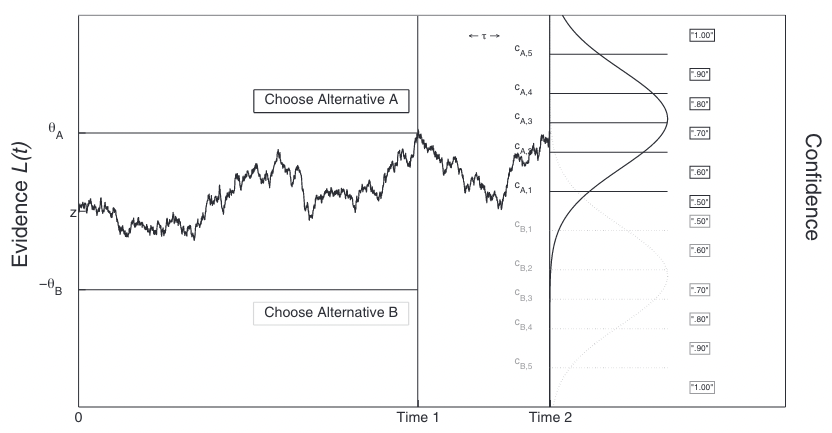
\includegraphics[width=1.0\linewidth]{images/pleskac2016.png}
\caption{Illustration de l'accumulation d'indices pour la décision et la confiance, extrait de \cite{pleskac_two-stage_2010}}
\label{fig:universe}
\end{figure}


\section*{Approche développée}

Sur la base de ces études, nous développons un agent artificiel associant apprentissage et prise de décision, capable de choix non binaires et dont le niveau de confiance dans ses décisions est estimé à l'aide d'un modèle à accumulateurs en compétition. Cet agent, conçu pour agir dans son environnement, pourra modifier son comportement sur la base de cette estimation. Nous discuterons également la possibilité d'utiliser ces évaluations pour offrir des garanties permettant de proposer un modèle digne de confiance par design. 

\bibliographystyle{plain}
\bibliography{biblio}



\end{document}

